% !TEX program = xelatex
\documentclass[UTF8,12pt,a4paper]{ctexart}
\usepackage[a4paper,top=2.25cm,bottom=2.20cm,left=2.30cm,right=2.30cm,headheight=15pt]{geometry}
\usepackage{amsmath,amssymb,bm,booktabs,tabularx,array,longtable,multirow}
\usepackage{graphicx,float,subcaption,xcolor,enumitem,fancyhdr,hyperref,setspace,titlesec}
\usepackage{siunitx}
\graphicspath{{../../05_figures/q1/}{../../05_figures/q2/}{../../05_figures/q3/}{../../05_figures/q4/}{../../05_figures/q5/}}

\definecolor{navy}{HTML}{17324D}
\definecolor{blue}{HTML}{2F6690}
\definecolor{teal}{HTML}{2A9D8F}
\definecolor{orange}{HTML}{E76F51}
\hypersetup{colorlinks=true,linkcolor=navy,citecolor=blue,urlcolor=blue,
  pdftitle={高性能芯片歧管式微通道热管理系统的多目标优化与鲁棒设计}}
\pagestyle{fancy}\fancyhf{}
\fancyhead[L]{高性能芯片热管理系统的优化}
\fancyhead[R]{数学建模论文修订稿}
\fancyfoot[C]{\thepage}
\renewcommand{\headrulewidth}{0.4pt}
\titleformat{\section}{\Large\bfseries\color{navy}}{\thesection}{0.7em}{}
\titleformat{\subsection}{\large\bfseries\color{blue}}{\thesubsection}{0.6em}{}
\setlist[itemize]{leftmargin=2em,itemsep=0.18em,topsep=0.22em}
\setlist[enumerate]{leftmargin=2.25em,itemsep=0.2em,topsep=0.22em}
\renewcommand{\arraystretch}{1.17}
\setstretch{1.10}
\setlength{\parindent}{2em}
\setlength{\parskip}{0.12em}

\newcommand{\Rth}{R_{\mathrm{th}}}
\newcommand{\dP}{\Delta p}
\newcommand{\mdotf}{\dot m}
\newcommand{\Vdot}{\dot V}
\newcommand{\ND}{\operatorname{ND}}
\newcommand{\CVaR}{\operatorname{CVaR}}

\title{\bfseries 高性能芯片歧管式微通道热管理系统的\\多目标优化与鲁棒设计}
\author{}
\date{}

\begin{document}
\maketitle
\vspace{-2.6em}

\begin{abstract}
针对高热流密度芯片歧管式微通道冷却系统，本文研究针肋宽度比$a$、歧管深高比$b$和针肋排数$N$对无量纲热阻$R$、压降$P$与温度非均匀性$U$的耦合影响，并依次完成机理分析、代理建模、多目标优化、偏好鲁棒和加工/工况鲁棒设计。

首先，根据有效过流面积、针肋侧表面积、局部阻力和支路供液平衡建立结构--性能机理链。由题设工况得到芯片热负荷为\SI{36}{W}，冷却液理想混合温升为\SI{8.61}{K}。附件84组数据的主效应与机理预测一致：增大$a$和$N$均存在换热强化与压降增加的竞争，增大$b$显著降低压降，但会改变局部换热与供液均匀性。

其次，将80个有针肋样本和4个无针肋样本视为两个不连通分支。有针肋分支比较二次OLS、三次OLS、三次Ridge与ARD--Mat\'ern高斯过程，最终选择三次Ridge；其$R,P,U$的重复折外NRMSE分别为$6.555\times10^{-6}$、0.004626和0.004333。无针肋分支仅采用四节点PCHIP保形插值，不作区间外预测。

随后，在Pareto偏序意义下，以401层析网格为确定性主搜索、分层NSGA-II为随机复核、差分进化和SLSQP作局部连续精化。最终名义折中解为$(a,b,N)=(0.224932,4.5,6)$，预测$(R,P,U)=(0.734330,0.097996,0.790195)$；其增强切比雪夫评分较最佳原始样本降低约10.05\%。对权重单纯形采用最小最大机会损失模型，$H=25,50,100$均得到同一偏好鲁棒解。

最后，将加工误差等效投影至$a,b$，分别采用LHS--CVaR和有界最坏情形两种鲁棒判据。两者均选择$N=6$、$b=4.4625$且$a\approx0.224$，说明推荐结构不依赖均匀分布假设。数值CVaR解为$(0.224006,4.4625,6)$，工程上推荐取$(0.224,4.4625,6)$或便于加工的$(0.225,4.4625,6)$。对于缺少变工况数据的流量与热负荷波动，本文只对固定候选结构进行压力测试，不将机理情景解释为精确最优设计。

\textbf{关键词：}歧管式微通道；Ridge响应面；Pareto优化；NSGA-II；最小最大遗憾；CVaR；鲁棒设计
\end{abstract}

\section{问题重述与总体思路}

研究对象为由歧管分配层和针肋微通道换热层构成的芯片液冷热管理系统。给定结构变量
\[
\bm x=(a,b,N)^{\mathrm T},\qquad
a=\frac{d_p}{w_c},\quad b=\frac{H_m}{H_c},
\]
其中$a$为针肋直径与通道宽度之比，$b$为歧管层与微通道层深高比，$N$为单个歧管单元内沿流向的针肋排数。三个无量纲响应$R,P,U$均越小越优，依次表征散热能力、泵功代价和温度均匀性/热点可靠性。

五个任务具有清晰递进关系。本文首先用传热与流动机理解释变量作用方向，再由附件数据建立代理模型；随后在代理模型上构造Pareto前沿并选择名义折中解；进而考察指标权重不确定性，最后将加工误差与运行波动纳入稳健性分析。整体路线为
\[
\text{机理分析}\longrightarrow\text{分段代理模型}\longrightarrow\text{Pareto优化}
\longrightarrow\text{偏好鲁棒}\longrightarrow\text{加工与工况鲁棒}.
\]

\section{模型假设与符号说明}

\subsection{基本假设}
\begin{enumerate}
  \item 系统处于稳态，冷却介质为单相不可压水，物性在题设工作区间内近似不变。
  \item 芯片热源均匀；不同结构方案采用相同热边界、入口总质量流量和外侧自然对流条件。
  \item 结构变化不改变芯片与衬底的主要固体导热路径，固体背景热阻可视为共同常量。
  \item 支路流量允许不均匀分配，且流量偏配是温度非均匀性的主要来源之一。
  \item 附件未说明改变$b=H_m/H_c$时具体保持哪一层尺寸不变。机理分析暂取$H_c$固定、由$H_m=bH_c$调节$b$；附件数据中的真实几何变化由代理模型统一学习。若改取总流体层高度$H_f=H_m+H_c$固定，则$H_m=bH_f/(1+b)$、$H_c=H_f/(1+b)$，但附件主效应仍显示$b$增大显著降低压降，故主要数据结论不依赖这一解释假设。
  \item 附件未公开三项无量纲指标的反归一化公式，故只在同一指标内比较相对变化，不把无量纲结果解释为真实温度或真实失效概率。
  \item 代理模型只在附件覆盖域内使用；有针肋与无针肋为不连通结构分支，不在两类结构之间插值。
\end{enumerate}

\subsection{主要符号}
\begin{table}[H]\centering\small
\caption{主要符号及含义}
\begin{tabularx}{\textwidth}{clX}
\toprule
符号&单位&含义\\\midrule
$a$&--&针肋宽度比$d_p/w_c$\\
$b$&--&歧管深高比$H_m/H_c$\\
$N$&--&沿流向针肋排数，取$2,4,6,8,10$\\
$R,P,U$&--&无量纲热阻、压降和温度非均匀性\\
$A_f,A_{wet}$&$\mathrm{m^2}$&有效过流面积与湿润换热面积\\
$\bm F^{\mathrm I}$&--&三目标理想点\\
$\bm F^{N,\mathrm{ref}}$&--&由合并参考前沿得到的参考Nadir点\\
$z_k$&--&第$k$项目标的归一化退让\\
$C_{\mathrm{AT}}$&--&等权增强切比雪夫评分\\
$r_{\mathrm{pref}}$&--&给定偏好权重下的机会损失\\
$\CVaR_{0.95}$&--&综合损失最差5\%尾部的条件均值\\
\bottomrule
\end{tabularx}
\end{table}

\section{结构参数与性能指标的机理模型}

\subsection{基础热量尺度}
芯片体积为$6\,\mathrm{mm}\times6\,\mathrm{mm}\times200\,\mu\mathrm m$。由题设体积热源和流量参数可得
\begin{equation}
Q=q'''V_c=36.0\ \mathrm W,\qquad
\Delta T_b=\frac{Q}{\mdotf c_p}=8.61\ \mathrm K.
\end{equation}
其中$\Delta T_b$仅为冷却液吸收全部热量后的理想混合温升，用于确定量级，不代表芯片最高温升。

\subsection{针肋几何、换热面积与流动阻力}
对有针肋结构，附件支持域为
\begin{equation}
\mathcal D_{\mathrm{pin}}=\{(a,b,N):0.1\le a\le0.3,\ 3\le b\le4.5,
\ N\in\{2,4,6,8,10\}\}.
\end{equation}
无针肋分支满足$(a,N)=(0,0)$且$3\le b\le4.5$。针肋宽度增加会缩小最小过流面积、增大间隙速度，同时扩大针肋换热面积：
\begin{align}
A_f(a)&=A_{f,0}-A_{\mathrm{block}}(a),\qquad
u_g(a)=\frac{\Vdot_{\mathrm{cell}}}{A_f(a)},\\
A_{\mathrm{pin,side}}(a,N)&\propto N\pi d_pH_c=N\pi aw_cH_c,\\
A_{wet}(a,N)&\approx A_{wet,0}+A_{\mathrm{pin,side}}(a,N).
\end{align}
$A_{\mathrm{pin,side}}$是针肋侧表面积的一阶近似，并非严格扣除针肋占据原壁面后的净新增面积。因此$a$同时引入“扩面强化”与“阻塞增阻”，而$N$增加换热作用次数并累积局部损失。

沿代表性主流路径，将系统压降分为歧管和微通道--针肋区两部分：
\begin{align}
\Delta p_{\mathrm{eq}}&\approx\Delta p_m(b)+\Delta p_c(a,N),\\
\Delta p_m&=\left[f_m\frac{L_m}{D_{h,m}}+K_m\right]\frac{\rho u_m^2}{2},\\
\Delta p_c&=\left[f_c\frac{L_c}{D_{h,c}}+K_{\mathrm{turn}}+N K_{\mathrm{pin}}(a)\right]
\frac{\rho u_g^2}{2}.
\end{align}
由于$A_m=W_mH_m=W_mbH_c$，增大$b$通常降低歧管速度和压降；增大$a,N$则提高微通道局部阻力。非线性交互由后续代理模型学习。

\subsection{热阻与温度非均匀性}
用特征温升定义物理热阻，并以有效换热面积解释结构趋势：
\begin{equation}
\Rth=\frac{T_{\max}-T_{in}}{Q},\qquad
\Rth\approx R_{\mathrm{solid}}+\frac{1}{h_{\mathrm{eff}}(a,b,N)A_{wet}(a,N)}.
\end{equation}
为表示歧管供液与微通道阻力的耦合，对第$j$条支路建立最简水力平衡
\begin{equation}
\Delta p_j=\mathcal R_j(a,N)\dot V_j+\frac{1}{2}\rho K_j(a,N)u_j^2,\qquad
u_j=\frac{\dot V_j}{A_j},\qquad\sum_j\dot V_j=\dot V.
\end{equation}
其中$\mathcal R_j$为支路线性水力阻力系数，单位为$\mathrm{Pa\cdot s/m^3}$。局部能量平衡为
\begin{equation}
\Delta T_{b,j}=\frac{Q_{up,j}}{\dot m_jc_p},\qquad
T_j-T_{in}\approx q_jR_{\mathrm{loc},j}+\Delta T_{b,j}.
\end{equation}
于是温度非均匀程度可概括为
\begin{equation}
\mathcal U=F\!\left(CV_{\dot m},CV_{R_{\mathrm{loc}}},CV_{\Delta T_b}\right),qquad
\frac{\partial F}{\partial CV_{\dot m}},
\frac{\partial F}{\partial CV_{R_{\mathrm{loc}}}},
\frac{\partial F}{\partial CV_{\Delta T_b}}\ge0.
\end{equation}
该局部单调关系表示：在其他条件相近时，流量、局部热阻或支路温升的离散程度增大，通常增加温度非均匀性。

\subsection{面向代理模型的物理启发特征}
为使机理分析与数据代理之间形成数学接口，由上述面积、阻塞、动压和供液关系构造
\begin{equation}
g_1=aN,\qquad g_2=a^2N,\qquad g_3=b^{-1},\qquad
g_4=b^{-2},\qquad g_5=\frac{aN}{b}.
\end{equation}
其中$g_1$近似表征针肋侧面积或强化总量，$g_2$近似表征投影阻塞量，
$g_3,g_4$对应歧管速度与动压尺度，$g_5$描述针肋阻力和歧管供液能力的交互。
本文将这些特征组成可解释Ridge对照模型；高精度三次Ridge仍作为正式优化代理，从而形成“机理特征负责解释、高精度模型负责优化”的双模型结构。

\subsection{数据趋势验证与指标合理性}
对80个有针肋全因子样本，定义因子$k$在水平$l$下的边际均值及相对偏差
\begin{equation}
\overline y_{k,l}=\frac{1}{n_{k,l}}\sum_{i:x_{ik}=l}y_i,qquad
\delta_{k,l}=\frac{\overline y_{k,l}-\overline y}{\overline y}\times100\%,
\quad y\in\{R,P,U\}.
\end{equation}
结果表明：$a=0.2$时$R,U$的边际均值最低，$a$从0.1增至0.3时$P$增大37.3\%；$b$从3增至4.5时$P$下降32.2\%，而$R$上升约1.94\%；$N$从2增至10时$R$下降2.18\%、$P$上升30.9\%，且考察水平中$N=4$的$U$边际均值最低。上述趋势与“强化换热--增大阻力--改变供液均匀性”的机理一致。

\begin{figure}[H]\centering
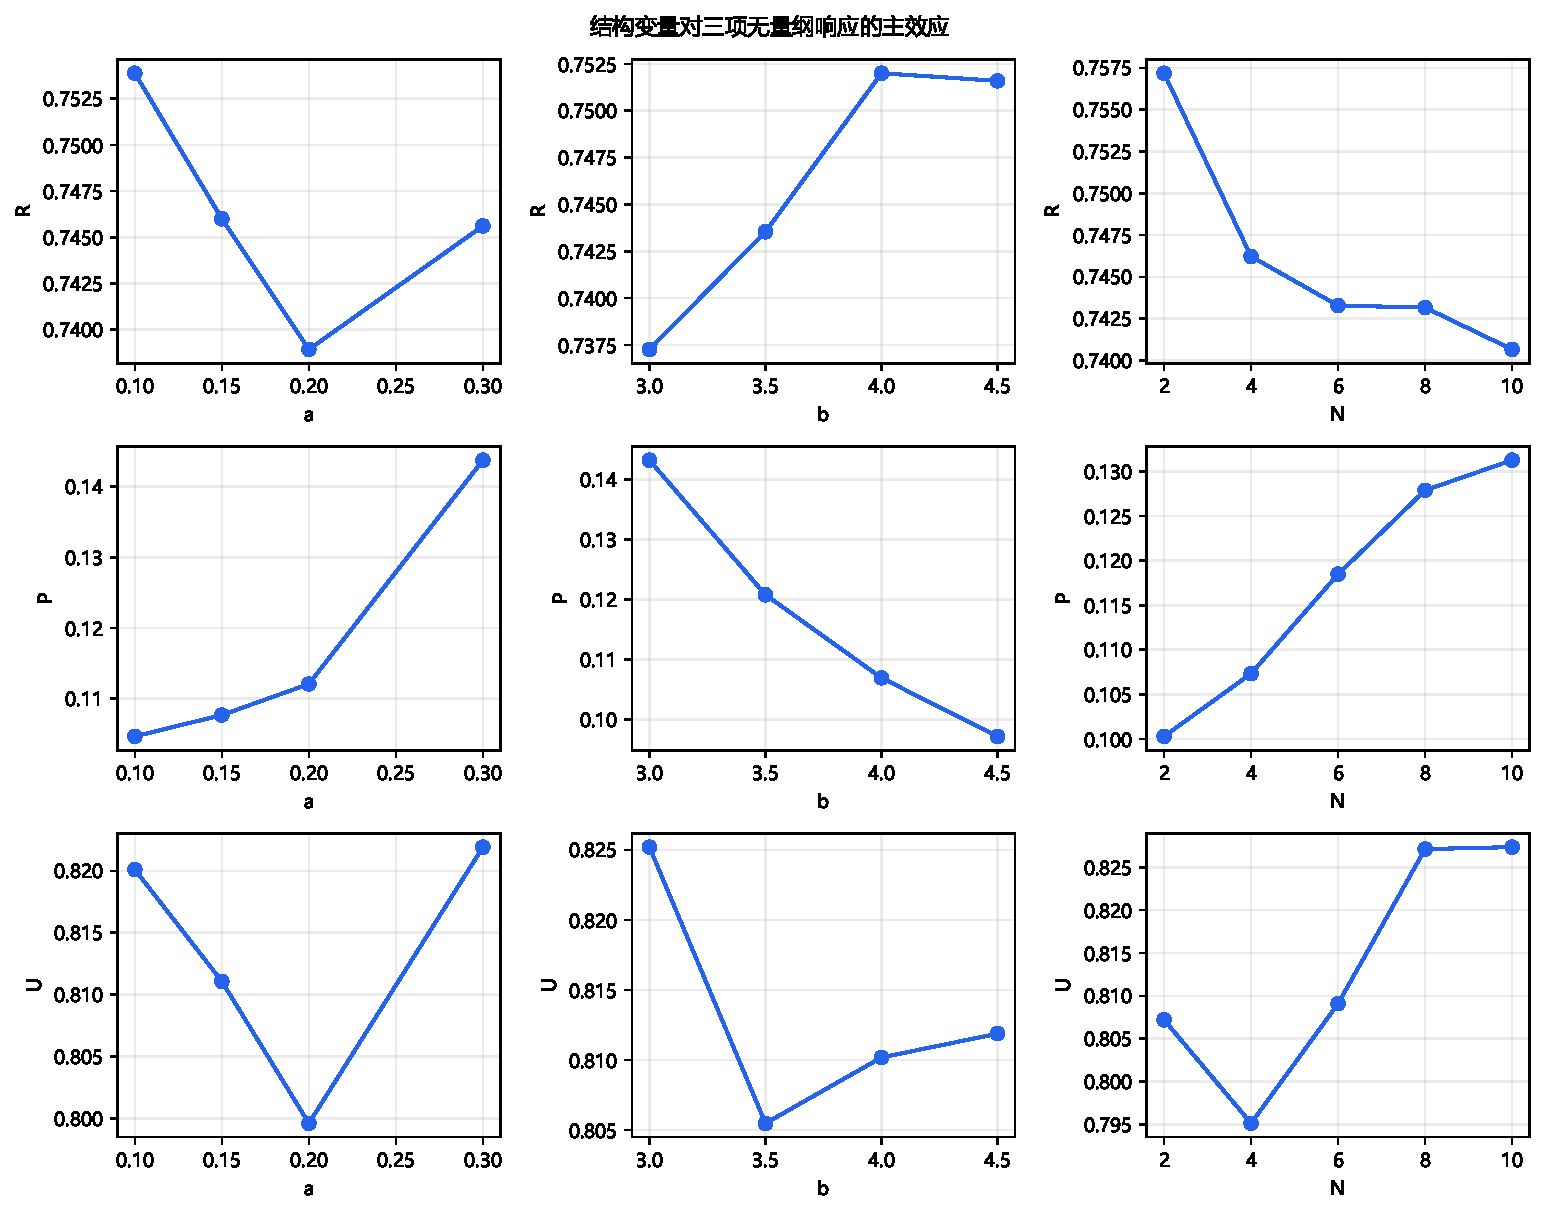
\includegraphics[width=.96\textwidth]{fig_q1_01_main_effects.pdf}
\caption{三个结构参数对三项性能指标的主效应；边际均值仅用于趋势解释，不代表联合最优。}
\end{figure}

由于80组有针肋样本是平衡$4\times4\times5$全因子设计，可进一步将确定性响应分解为
\begin{equation}
y_{ijk}=\mu+A_i+B_j+C_k+(AB)_{ij}+(AC)_{ik}+(BC)_{jk}+(ABC)_{ijk},
\end{equation}
并以$\eta_S^2=SS_S/SS_T$度量各效应贡献率。这里不进行$p$值检验，因为附件数据是确定性计算结果而非含重复误差的随机实验。

\begin{table}[H]\centering\small
\caption{全因子主效应与交互效应贡献率（\%）}
\begin{tabular}{crrrrrrr}
\toprule
响应&$a$&$b$&$N$&$a\times b$&$a\times N$&$b\times N$&三阶交互\\\midrule
$R$&23.87&31.80&28.71&0.65&5.94&6.07&2.97\\
$P$&31.70&38.89&18.13&0.00&11.25&0.01&0.01\\
$U$&24.29&16.66&48.00&6.24&2.42&2.24&0.14\\
\bottomrule
\end{tabular}
\end{table}
热阻同时受$b,N,a$三个主效应控制，最大的二阶交互为$b\times N$；压降主要由$b$和$a$控制，且$a\times N$贡献达11.25\%，定量反映针肋阻塞与排数累积；温度非均匀性则由$N$主导，$a\times b$是最大二阶交互。该分解既证明了交互项的必要性，也解释了不同$N$层形成不同Pareto分支的原因。

\begin{figure}[H]\centering
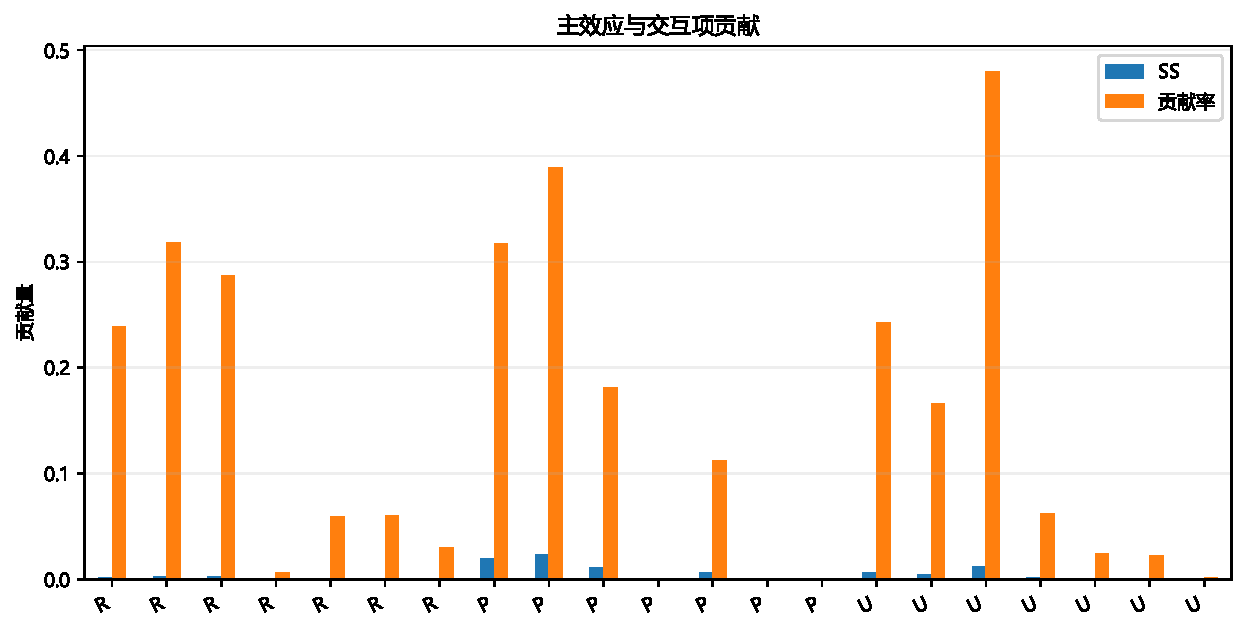
\includegraphics[width=.82\textwidth]{fig_q1_03_anova_contributions.pdf}
\caption{三项响应的全因子效应贡献率。}
\end{figure}

$R,P,U$分别对应散热能力、泵功代价与热点可靠性。固定体积流量时
\begin{equation}
W_{\mathrm{pump}}=\frac{\Delta p\,\dot V}{\eta_p}\propto\Delta p,
\end{equation}
而相近的$R,P$仍可对应不同$U$，因此三项指标不可互相替代，均应保留在多目标模型中。

\section{分段代理模型的建立与检验}

\subsection{数据分支与候选模型}
附件共84组确定性结果，其中80组有针肋样本构成$4\times4\times5$平衡全因子设计，另4组为无针肋节点。由于不存在$a=0,N>0$或$a>0,N=0$的合法结构，定义分段模型
\begin{equation}
\widehat y_k(a,b,N)=
\begin{cases}
\widehat y_{k,0}(b),&(a,N)=(0,0),\\
\widehat y_{k,1}(a,b,N),&(a,b,N)\in\mathcal D_{\mathrm{pin}}.
\end{cases}
\end{equation}
无针肋分支仅采用四节点PCHIP保形插值，其节点为
\begin{equation}
\begin{array}{c|ccc}
b&R&P&U\\\hline
3.0&0.740827&0.123952&0.873100\\
3.5&0.754456&0.102276&0.838862\\
4.0&0.767907&0.088704&0.838398\\
4.5&0.770128&0.078985&0.844634
\end{array}.
\end{equation}
由于只有4个样本，该支路不声称具有独立预测能力，也不用于区间外推。

对有针肋输入先标准化$\xi_j=(x_j-\mu_j)/s_j$，再构造完整三次多项式特征$\bm\phi_3(\bm\xi)$。Ridge模型写为
\begin{equation}
(\widehat\beta_{0k},\widehat{\bm\beta}_k)=
\arg\min_{\beta_0,\bm\beta}
\left\{\left\|\bm y_k-\beta_0\bm 1-\bm X_{\phi}\bm\beta\right\|_2^2
+\lambda_k\|\bm\beta\|_2^2\right\}.
\end{equation}
截距不参与正则化。输入变量先标准化，构造的多项式特征再在训练折内标准化，形成两阶段标准化流程。

\subsection{验证方案与模型选择}
外层使用5折交叉验证并重复10次，内层5折选择$\lambda_k$；所有标准化、特征构造和参数选择均限制在训练折内。每个样本在10次重复中得到10个折外预测，取平均后绘制OOF预测图；误差统计则先按每次重复计算，再汇总均值和标准差。另逐一留出$a,b,N$的13个因子水平，区分内部水平插值和边界水平外推压力测试。

\begin{table}[H]\centering\small
\caption{候选代理模型的重复折外NRMSE}
\begin{tabular}{lrrr}
\toprule
模型&$R$&$P$&$U$\\\midrule
二次OLS&0.097299&0.025243&0.126270\\
三次OLS&$6.559\times10^{-6}$&0.004626&0.004335\\
三次Ridge&$6.555\times10^{-6}$&0.004626&0.004333\\
ARD--Mat\'ern GP&0.009000&0.007726&0.016534\\
\bottomrule
\end{tabular}
\end{table}

三次OLS与Ridge精度几乎相同，三次设计矩阵SVD条件数为14.098，无严重病态。考虑对高阶项施加轻微约束并统一后续优化接口，最终三个响应均采用三次Ridge。确定模型族后，使用全部80个有针肋样本重新进行5折交叉验证选择$\lambda_k$，再在全样本上拟合并输出最终系数。

\subsection{离散排数编码与机理特征对照}
把$N$作为数值坐标进入三次多项式，隐含五种排数之间具有平滑有序关系。为检验该结构假设，本文增加两类对照：其一将$N$作one-hot类别变量，并与$(a,b)$三次特征交互；其二对每个$N$层分别拟合二维三次Ridge。另以$(g_1,\ldots,g_5)$建立机理特征Ridge。四类模型使用相同的10次重复5折划分。

\begin{table}[H]\centering\small
\caption{不同排数编码与机理特征模型的重复折外NRMSE}
\begin{tabular}{lrrr}
\toprule
模型&$R$&$P$&$U$\\\midrule
$N$数值编码三次Ridge&$6.64\times10^{-6}$&0.00460&0.00424\\
$N$类别编码及交互&0.00576&0.00801&0.01496\\
按$N$分层响应面&0.04431&0.01306&0.09729\\
五项机理特征Ridge&0.12671&0.03650&0.19440\\
\bottomrule
\end{tabular}
\end{table}
数值编码的精度最高；类别编码和分层响应面虽然误差较大，但三者各自在全域重新优化后均选择$N=6$，且$a^*$分别为0.224932、0.224843、0.224810，$b^*$均为4.5。由此可见，最优排数不依赖$N$的编码方式。机理特征模型精度明显较低，不替代正式代理；其价值在于把Q1的面积、阻塞和供液尺度转化为可计算的解释性基准。

\begin{table}[H]\centering\small
\caption{最终三次Ridge模型的折外性能与复现参数}
\begin{tabular}{crrrr}
\toprule
响应&$\lambda_k$&$R^2_{\mathrm{OOF}}$&OOF-NRMSE&MaxAE\\\midrule
$R$&$10^{-5}$&接近1&$6.555\times10^{-6}$&$7.631\times10^{-7}$\\
$P$&$10^{-2}$&0.999548&0.004626&0.004200\\
$U$&$10^{-3}$&0.999679&0.004333&0.001817\\
\bottomrule
\end{tabular}
\end{table}

留一水平测试中，内部插值的最大NRMSE为$(0.0881,0.0445,0.1195)$，边界外推则增至$(2.0595,0.3965,2.1200)$。最严重的$R,U$边界外推来自留出$a=0.30$，$P$来自留出$b=4.50$；内部插值中$R,U$对$a=0.20$较敏感，$P$对$b=4.00$较敏感。因此本文严格禁止在$a>0.3$、$b>4.5$等区域使用代理模型。

进一步将每个$(a_i,b_j)$位置对应的五个$N$样本同时留出，共进行16次结构化测试。总体NRMSE为$6.90\times10^{-6}$、0.00437和0.00492；最差单个组合的NRMSE为$1.08\times10^{-5}$、0.01473和0.01093。该结果更接近连续优化中的二维几何插值任务，说明模型并非只依靠同一$(a,b)$位置上的其他排数样本。

$R$的折外误差低至$10^{-6}$量级，表明附件热阻数据在规则网格上近似满足低阶代数结构。由于预处理严格限制在训练折内，该结果不是全数据标准化造成的泄漏；但它只说明样本域内插值稳定，不意味着设计域外同样具有近乎精确的预测能力，其误差也已接近原始数据保留小数精度。

最终显式模型为
\begin{equation}
\widehat y_k=\beta_{0k}+\sum_{q=1}^{19}\beta_{qk}
\frac{\phi_q(\bm\xi)-m_q}{t_q},
\quad k\in\{R,P,U\},
\end{equation}
其输入标准化参数和三个响应的截距分别为
\begin{align}
\bm\mu_x&=(0.1875,3.75,6)^{\mathrm T},\qquad
\bm s_x=(0.073951,0.559017,2.828427)^{\mathrm T},\\
(\beta_{0R},\beta_{0P},\beta_{0U})
&=(0.746101800,0.1170519125,0.8131816625).
\end{align}
完整系数与特征尺度见附录。

\section{多目标优化与名义最优设计}

\subsection{Pareto模型与统一尺度}
多目标问题规范写为
\begin{equation}
\min_{\bm x\in\mathcal D}^{\mathrm{Pareto}}\bm F(\bm x),\qquad
\bm F(\bm x)=\left(\widehat R(\bm x),\widehat P(\bm x),\widehat U(\bm x)\right)^{\mathrm T}.
\end{equation}
该式表示在Pareto偏序意义下寻找非支配解，而非把三个数值直接按普通标量比较。由三个单目标锚点获得理想点，并基于401网格、20次NSGA-II和局部精化的合并参考前沿得到数值参考Nadir点：
\begin{align}
\bm F^{\mathrm I}&=(0.720227,0.076040,0.771787)^{\mathrm T},\\
\bm F^{N,\mathrm{ref}}&=(0.760176,0.158555,0.819442)^{\mathrm T}.
\end{align}
后者是有限参考集上的近似最劣点，不宣称为解析意义上的精确Nadir点。归一化目标为
\begin{equation}
z_k(\bm x)=\frac{F_k(\bm x)-F_k^{\mathrm I}}
{F_k^{N,\mathrm{ref}}-F_k^{\mathrm I}}.
\end{equation}

\subsection{多算法搜索与收敛性}
鉴于仅有两个连续变量和一个低基数离散变量，正式方法压缩为三层：
\begin{itemize}
  \item 对每个合法$N$在$(a,b)$平面实施101、201和401三级致密网格，作为确定性主搜索；
  \item 对五个$N$层分别运行NSGA-II，20个独立随机种子用于随机复核；
  \item 以网格和NSGA-II折中点为初值，进行一次全局--局部连续精化，以消除网格步长误差。
\end{itemize}
统一参考集为
\begin{equation}
\mathcal P_{\mathrm{ref}}=\ND\!\left(\mathcal P_{401}\cup
\bigcup_{r=1}^{20}\mathcal P_{\mathrm{NSGA},r}\cup\mathcal P_{\mathrm{local}}\right),
\end{equation}
共含18183个非支配点。采用精确三维超体积HV、IGD+和Spacing比较覆盖度与均匀性。

\begin{table}[H]\centering\small
\caption{候选优化算法的统一比较}
\begin{tabular}{lrrrrrr}
\toprule
方法&非支配点&HV&IGD+&Spacing&时间/s&评价次数\\\midrule
101网格&1362&0.902914&0.001239&0.002824&0.96&53006\\
201网格&4679&0.903767&0.000503&0.001314&2.94&204006\\
401网格&16858&0.904148&0.000014&0.000624&10.13&806006\\
NSGA-II均值&107.95&0.892203&0.011923&0.017331&0.94&15300\\
NSGA-II标准差&3.05&0.001348&0.002173&0.002833&0.08&--\\
\bottomrule
\end{tabular}
\end{table}
201到401网格的HV相对变化为$4.21\times10^{-4}<10^{-3}$。运行时间只反映本文实现环境，不作为算法理论效率的直接比较依据。NSGA-II以约1.9\%的网格评价次数找到相同折中区域，表明结果不依赖单一搜索算法。

前沿的结构规律比算法指标更重要：$N=2$的局部阻力最小，因而占据低压降端，但热阻偏高；$N=4$在附件中给出最低温度非均匀性，是均温偏好下的主要层；$N=6$兼顾热阻、压降和均匀性，形成等权折中；$N=8,10$只有在散热权重较大时进入最优区域。多数折中解取较大的$b$，是因为附件中$b$增大带来的降压收益显著，而热阻代价相对较小；这只是在$b\le4.5$数据域内的权衡，不能向域外延伸。

\begin{figure}[H]\centering
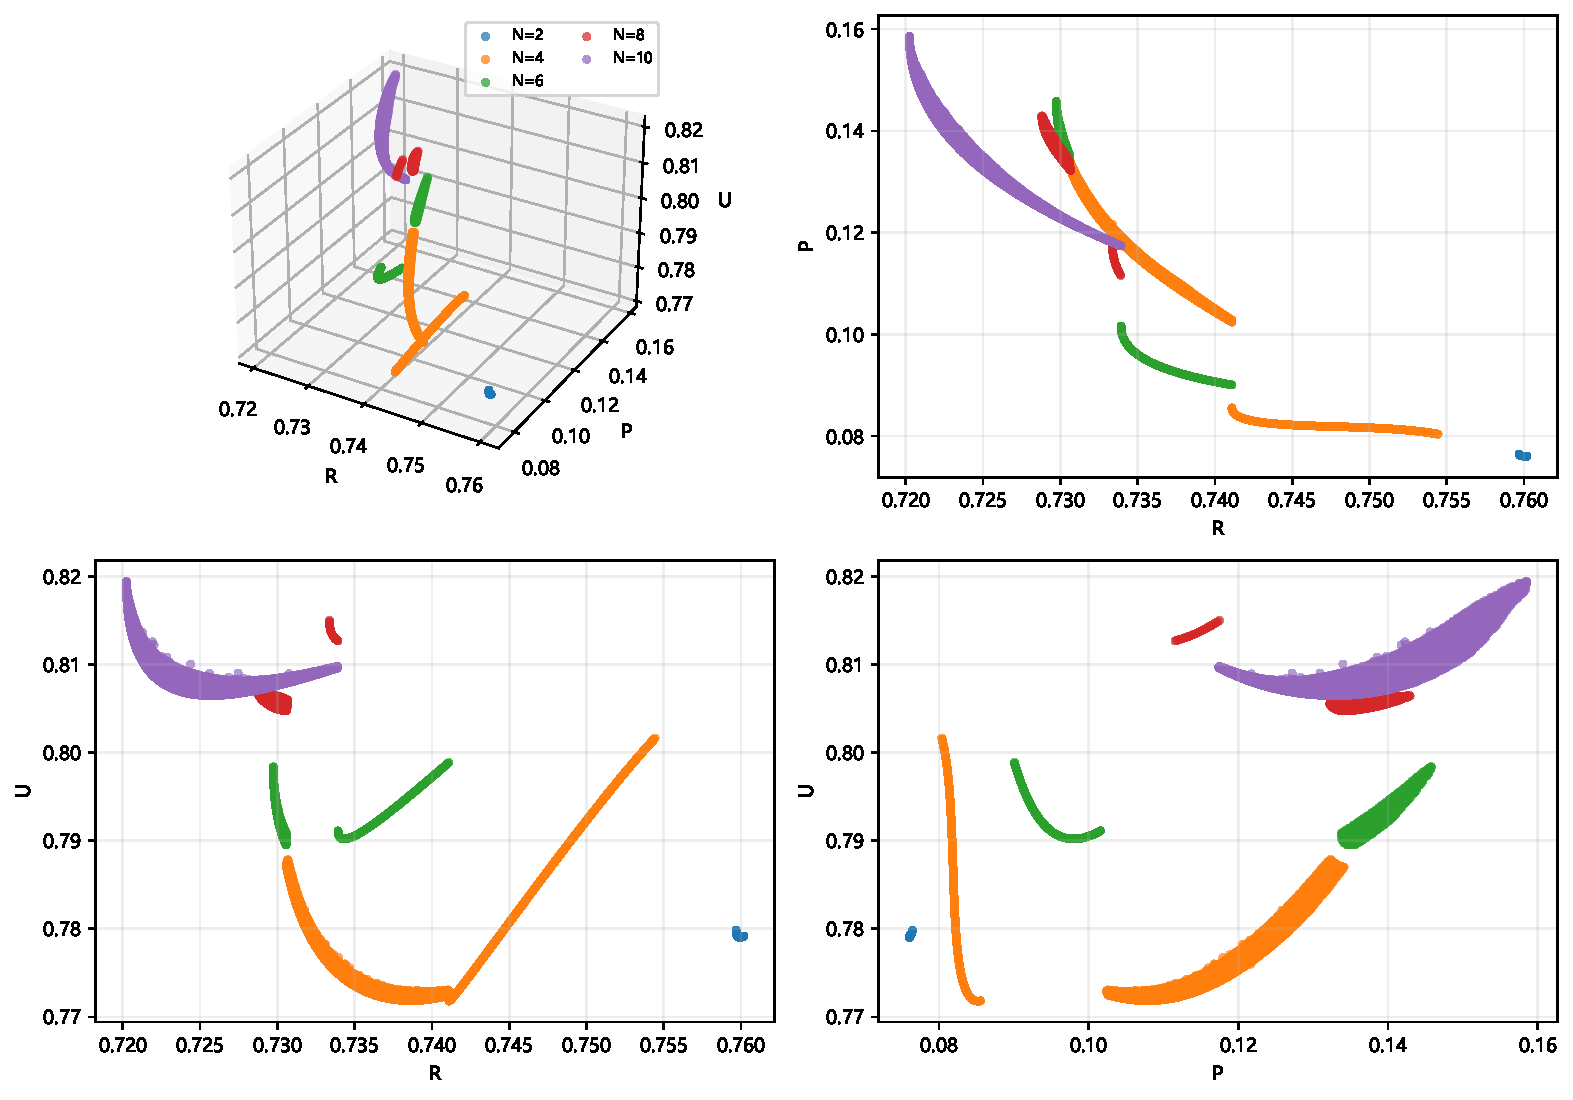
\includegraphics[width=.95\textwidth]{fig_q3_01_pareto_front.pdf}
\caption{合并参考Pareto前沿及其两两投影。无针肋节点在全局合并后均被支配。}
\end{figure}

401网格得到16858个全局非支配点；2001个无针肋候选在各自分支内部虽均非支配，但全局合并后保留0个。即使不依赖PCHIP连续插值，四个原始无针肋节点也均被至少一个有针肋原始样本支配。

\subsection{等权折中与结果审计}
采用等权增强切比雪夫准则
\begin{equation}
C_{\mathrm{AT}}(\bm x)=\max\{z_R,z_P,z_U\}
+10^{-4}(z_R+z_P+z_U).
\end{equation}
主项控制最差标准化退让，增强项仅用于打破并列。连续精化得到
\begin{equation}
\boxed{\bm x_{\mathrm{nom}}^*=(0.224932,4.500000,6)},\qquad
(R,P,U)=(0.734330,0.097996,0.790195).
\end{equation}
与最佳原始样本$(0.2,4.5,6)$相比，$C_{\mathrm{AT}}$由0.4295降至0.3864，下降约10.05\%。原始样本行采用附件计算值，其余连续设计采用Ridge预测值。

仅在同一最终点比较预测值不足以检验优化稳定性，因此本文让不同模型各自重新优化，并定义模型集合保守响应
\begin{equation}
F_k^{\mathrm{con}}(\bm x)=\max_{m\in\{\mathrm{Ridge,OLS,GP}\}}
\widehat F_{k,m}(\bm x).
\end{equation}

\begin{table}[H]\centering\small
\caption{不同代理模型各自重新优化及保守审计}
\begin{tabular}{lrrrr}
\toprule
模型&$a^*$&$b^*$&$N^*$&综合评分\\\midrule
三次Ridge&0.224932&4.5000&6&0.38638\\
三次OLS&0.224942&4.5000&6&0.38628\\
Mat\'ern GP&0.220471&4.5000&6&0.39555\\
$N$类别编码Ridge&0.224843&4.5000&6&0.38798\\
按$N$分层响应面&0.224810&4.5000&6&0.38888\\
模型集合保守解&0.220471&4.5000&6&0.39555\\
\bottomrule
\end{tabular}
\end{table}
六种结果均选择$N=6$且$b=4.5$，$a^*$位于$[0.2205,0.2249]$。因此推荐结构不仅对搜索算法稳定，也对代理形式和排数编码稳定。将$a$在Ridge最优点附近加减0.005时评分分别约为0.3885和0.3884；相邻排数$N=4,8$的评分为0.5227和0.8517，说明排数选择比小幅连续参数扰动更敏感。由于$b=4.5$位于数据边界，只能说明域内边界最优，不能外推$b>4.5$仍会改善。

\section{权重变化与偏好鲁棒设计}

对权重$\bm w=(w_R,w_P,w_U)$，定义
\begin{equation}
G(\bm x;\bm w)=\max_k\{3w_kz_k(\bm x)\}
+10^{-4}\sum_k3w_kz_k(\bm x),\quad w_k\ge0,\quad\sum_kw_k=1.
\end{equation}
系数3仅用于使等权$w_k=1/3$时$G$与问题3的$C_{\mathrm{AT}}$完全一致；它不改变每组权重下的最优方案，只统一缩放评分和遗憾值。

对给定权重，令$G^*(\bm w)=\min_{\bm x\in\mathcal P_{\mathrm{ref}}}G(\bm x;\bm w)$，定义偏好机会损失
\begin{equation}
r_{\mathrm{pref}}(\bm x,\bm w)=G(\bm x;\bm w)-G^*(\bm w).
\end{equation}
在离散权重单纯形
\begin{equation}
\mathcal W_H=\left\{\left(\frac{i}{H},\frac{j}{H},\frac{k}{H}\right):
i,j,k\in\mathbb Z_{\ge0},\ i+j+k=H\right\}
\end{equation}
上求解最小最大遗憾模型
\begin{equation}
\bm x_{\mathrm{pref}}^{\mathrm{rob}}=
\arg\min_{\bm x\in\mathcal P_{\mathrm{ref}}}
\max_{\bm w\in\mathcal W_H}r_{\mathrm{pref}}(\bm x,\bm w).
\end{equation}

\begin{table}[H]\centering\small
\caption{代表性偏好及其专属最优方案}
\begin{tabular}{lcrrrr}
\toprule
场景&$(w_R,w_P,w_U)$&$a$&$b$&$N$&$G$\\\midrule
均衡&$(1/3,1/3,1/3)$&0.2249&4.5000&6&0.38638\\
散热优先&$(0.6,0.2,0.2)$&0.2173&3.3746&8&0.43223\\
能耗优先&$(0.2,0.6,0.2)$&0.2276&4.5000&4&0.31344\\
均匀性优先&$(0.2,0.2,0.6)$&0.2172&3.4315&4&0.25082\\
热可靠性优先&$(0.45,0.10,0.45)$&0.2414&3.0411&4&0.36148\\
\bottomrule
\end{tabular}
\end{table}
各行$G$对应不同权重，只能在场景内部解释。$H=25,50,100$分别含351、1326和5151组权重，均得到
\begin{equation}
\boxed{\bm x_{\mathrm{pref}}^{\mathrm{rob}}=(0.224932,4.5,6)},\qquad
\max r_{\mathrm{pref}}=1.15896.
\end{equation}
遗憾是评分差值而非概率量，故可以大于1。等权名义最优恰好也是最小最大遗憾解，这是计算结果而非预设，说明该方案处于多个偏好区域的相对中心位置。$H=50$时$N=2,4,6,8,10$的最优区域占比分别为3.8\%、55.8\%、22.7\%、2.6\%、15.0\%；$N=4$覆盖场景最多，而$N=6$控制最坏损失更优，两者判据不同。

上述区域占比默认权重单纯形采用均匀面积测度。为检验绝对评分尺度和极端权重的影响，再定义归一化相对遗憾
\begin{equation}
r_{\mathrm{rel}}(\bm x,\bm w)=
\frac{G(\bm x;\bm w)-G^*(\bm w)}
{G^{\max}(\bm w)-G^*(\bm w)+10^{-12}},
\end{equation}
并比较完整单纯形与温和权重域$\mathcal W_{0.1}=\{\bm w:w_k\ge0.1,\sum_kw_k=1\}$。

\begin{table}[H]\centering\small
\caption{遗憾定义与权重不确定域敏感性}
\begin{tabular}{llrrrr}
\toprule
权重域&判据&权重数&$a$&$b$&$N$\\\midrule
完整单纯形&绝对遗憾&1326&0.224932&4.5000&6\\
完整单纯形&相对遗憾&1326&0.224932&4.5000&6\\
$w_k\ge0.1$&绝对遗憾&666&0.217000&3.4500&4\\
$w_k\ge0.1$&相对遗憾&666&0.224932&4.5000&6\\
\bottomrule
\end{tabular}
\end{table}
完整单纯形下两种遗憾均选择$N=6$；温和权重域中的相对遗憾也保持$N=6$，但绝对遗憾转向$N=4$。这说明“$N=6$对全部偏好定义都唯一鲁棒”并不成立。本文把$N=6$作为兼顾极端场景和相对损失的主推荐，同时把$N=4$列为应用偏好明确排除极端权重时的备选。

\begin{figure}[H]\centering
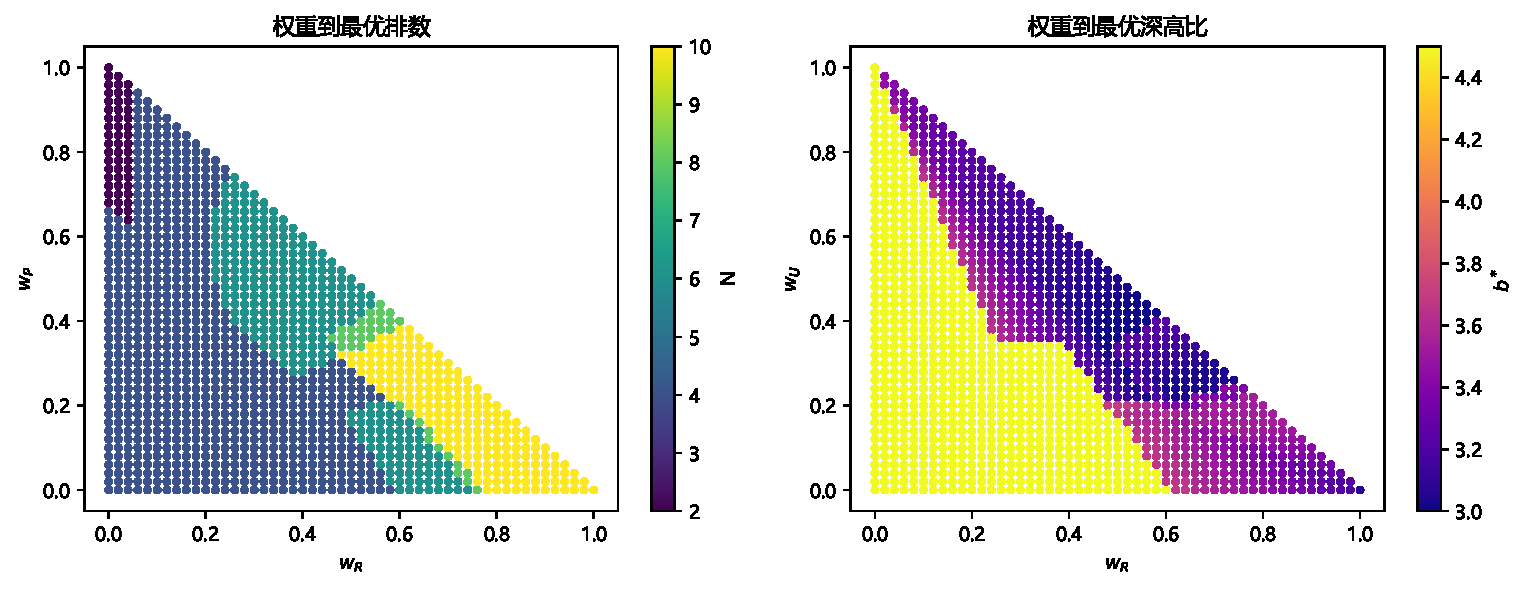
\includegraphics[width=.88\textwidth]{fig_q4_01_weight_mapping.pdf}
\caption{权重到最优结构的映射。}
\end{figure}

\section{加工误差与工况波动下的鲁棒性}

\subsection{加工误差：数据支持下的A类结论}
题目未给出真实制造公差分布，故首先采用参数化等效公差模型
\begin{equation}
\varepsilon_a,\varepsilon_b\sim U[-0.025,0.025],\qquad
a^r=a+0.20\varepsilon_a,\quad b^r=b+1.50\varepsilon_b.
\end{equation}
这对应$|\Delta a|\le0.005$、$|\Delta b|\le0.0375$。$N$为整数加工决策，不作连续扰动。为保证所有实现值均处于代理模型支持域，名义设计必须位于收缩可行域
\begin{equation}
\boxed{\mathcal D_{\mathrm{rob,pin}}=
\{(a,b,N):0.105\le a\le0.295,\ 3.0375\le b\le4.4625,
\ N\in\{2,4,6,8,10\}\}}.
\end{equation}

该模型中的误差直接作用于比值，不能解释为真实制造尺寸服从均匀分布。获得工艺公差后，应改用物理尺寸传播
\begin{equation}
a^r=\frac{d_p+\Delta d_p}{w_c+\Delta w_c},\qquad
b^r=\frac{H_m+\Delta H_m}{H_c+\Delta H_c},
\end{equation}
并允许同一工序造成的相关误差。附件没有给出$w_c,H_c$的数值，故目前只能将工程比值写为$d_p=0.224w_c$、$H_m=4.4625H_c$，不能可靠换算为微米尺寸。若制造步长为$\Delta d$，还应取
\begin{equation}
d_p^{\mathrm{fab}}=\operatorname{round}\!\left(\frac{d_p^*}{\Delta d}\right)\Delta d
\end{equation}
并重新评价离散化损失。

对每个候选，用固定随机种子的LHS样本传播误差，定义
\begin{equation}
C_{\mathrm{str}}=\max_kz_k\!\left(\widehat{\bm F}(\bm x^r)\right)
+10^{-4}\sum_kz_k\!\left(\widehat{\bm F}(\bm x^r)\right),
\end{equation}
并最小化尾部风险
\begin{equation}
\CVaR_{0.95}(C)=\mathbb E[C\mid C\ge\operatorname{VaR}_{0.95}(C)].
\end{equation}
名义点$b=4.5$在双侧公差下约有50\%实现值越出代理域，因此不对其越域结果作正式CVaR比较。将其投影至可行边界得到
$\bm x_{\mathrm{proj}}=(0.224932,4.4625,6)$。

\begin{table}[H]\centering\small
\caption{鲁棒可行域内的加工风险比较（$L=20000$）}
\begin{tabular}{lrrrrrr}
\toprule
方案&$a$&$b$&$N$&名义评分&Q95&CVaR95\\\midrule
名义可行投影&0.224932&4.4625&6&0.40444&0.41817&0.41907\\
结构鲁棒解&0.224006&4.4625&6&0.40443&0.41813&0.41893\\
\bottomrule
\end{tabular}
\end{table}
结构鲁棒解相对投影方案的CVaR仅下降约0.04\%，说明两者工程上近乎等价；真正关键的是将$b$从4.5内移至4.4625，而非$a$的第四至第六位小数。

\begin{table}[H]\centering\small
\caption{结构鲁棒解的LHS样本量与扰动幅度复核}
\begin{tabular}{ccccc}
\toprule
项目&样本量/幅度&$a$&$b$&CVaR95\\\midrule
样本量复核&20000&0.224006&4.4625&0.418925\\
样本量复核&40000&0.224006&4.4625&0.418930\\\midrule
小扰动&$\delta=0.010$&0.224530&4.4850&0.400891\\
中扰动&$\delta=0.025$&0.224006&4.4625&0.418925\\
大扰动&$\delta=0.050$&0.223222&4.4250&0.441107\\
\bottomrule
\end{tabular}
\end{table}
样本量加倍后的绝对变化约$5.3\times10^{-6}$；在三档扰动中$N=6$保持不变，且$b$随允许扰动增大按鲁棒边界向内移动。幅度复核采用同一代理模型和固定LHS种子，属于参数化敏感性证据，不代表真实加工标准。

由于题目只给出“小范围扰动”而未指定概率分布，同时建立不依赖分布的有界最坏情形模型
\begin{equation}
\bm x_{\mathrm{wc}}=
\arg\min_{\bm x\in\mathcal D_{\mathrm{rob,pin}}}
\max_{(\delta_a,\delta_b)\in\mathcal U}
C_{\mathrm{AT}}(a+\delta_a,b+\delta_b,N),
\end{equation}
其中$\mathcal U=\{(\delta_a,\delta_b):|\delta_a|\le0.005,
|\delta_b|\le0.0375\}$。对扰动矩形作致密网格扫描，并在各$N$层连续精化，得到
\begin{equation}
\bm x_{\mathrm{wc}}=(0.223899,4.4625,6),\qquad
\max_{\delta\in\mathcal U}C_{\mathrm{AT}}=0.42077.
\end{equation}

\begin{table}[H]\centering\small
\caption{概率尾部与有界最坏情形双鲁棒判据}
\begin{tabular}{lrrrr}
\toprule
判据&$a$&$b$&$N$&风险值\\\midrule
均匀等效公差下CVaR&0.224006&4.4625&6&0.41893\\
有界最坏情形&0.223899&4.4625&6&0.42077\\
\bottomrule
\end{tabular}
\end{table}
两种判据对$a$的差异仅$1.07\times10^{-4}$，并共同选择$N=6$和鲁棒边界$b=4.4625$。因此最终推荐不依赖均匀分布假设；CVaR强调最差5\%的平均损失，最坏情形模型则更保守地控制所有有界扰动。

带符号标准回归系数
\begin{equation}
\mathrm{SRC}_{kj}=\widehat\beta_{kj}\frac{\sigma_{X_j}}{\sigma_{Y_k}}
\end{equation}
表明$\varepsilon_b$主导综合评分；加工误差下单项响应的线性近似$R^2$均不低于0.992。SRC只用于识别局部方向和主导因素，不解释为严格方差贡献率。

\subsection{运行工况：机理假设下的B类情景}
附件没有不同流量、热负荷下的CFD或实验样本，因此工况波动只能作为机理情景。令$s_m,s_q\sim U[0.95,1.05]$分别表示流量与热负荷缩放，定义
\begin{align}
P^{\mathrm{op}}&=\widehat P(\bm x^r)[\alpha_Ps_m+(1-\alpha_P)s_m^2],\\
R^{\mathrm{op}}&=\widehat R(\bm x^r)[\theta_R+(1-\theta_R)s_m^{-m_R}],
\qquad\Theta_R=s_qR^{\mathrm{op}},\\
U_A^{\mathrm{op}}&=\widehat U(\bm x^r)s_m^{-m_U},\qquad
U_B^{\mathrm{op}}=\widehat U(\bm x^r)s_qs_m^{-m_U}.
\end{align}
三档机理参数取
\begin{center}
\begin{tabular}{lrrrrl}\toprule
情景&$\alpha_P$&$\theta_R$&$m_R$&$m_U$&解释\\\midrule
S1&0.80&0.75&0.25&0.25&弱流量敏感\\
S2&0.50&0.50&0.50&0.50&中等混合机制\\
S3&0.20&0.25&0.80&0.80&强流量敏感\\\bottomrule
\end{tabular}
\end{center}

为避免对未标定机理情景给出过度精确的“最优结构”，本节改作压力测试。固定四类候选：名义可行投影$(0.224932,4.4625,6)$、加工鲁棒方案$(0.224006,4.4625,6)$、$N=4$代表方案$(0.241,3.08,4)$和$N=10$代表方案$(0.223,3.45,10)$。在S1--S3及$U$模型A/B共六个情景中比较CVaR范围、观测到的最大评分及相对各情景最优值的最大遗憾。

\begin{table}[H]\centering\small
\caption{固定候选结构的工况压力测试}
\begin{tabular}{lrrrr}
\toprule
候选结构&最小CVaR&最大CVaR&最大评分&最大遗憾\\\midrule
名义可行投影&1.2573&1.6259&1.9531&0.2907\\
加工鲁棒方案&1.2586&1.6260&1.9538&0.2920\\
$N=4$代表方案&1.1544&1.4782&1.7804&0.1878\\
$N=10$代表方案&0.9704&1.9820&2.3078&0.5243\\
\bottomrule
\end{tabular}
\end{table}
$U$模型A下大排数方案更有利，而模型B下中等排数方案更稳健；跨全部假设包络时，$N=4$代表方案的最大遗憾较小，$N=10$虽在部分情景表现最好却对模型形式最敏感。由于排数选择随外推形式改变，现有数据不足以支持把正式推荐从$N=6$改为4或10。待获得变流量、变热负荷数据后，应重新训练联合代理模型，而不是继续细化这些情景中的小数位。

\section{模型评价、结论与工程建议}

\subsection{模型优点}
\begin{enumerate}
  \item 形成了从物理机理、统计代理、Pareto搜索到两类鲁棒性的完整闭环，且每一步均受附件数据域约束。
  \item 显式区分有针肋与无针肋分支、连续变量与离散排数，避免生成物理非法结构。
  \item 利用平衡全因子设计定量分解主效应和交互效应，并以物理启发特征连接机理与代理模型。
  \item 采用重复折外验证、$(a,b)$组合留出、排数编码对照、不同代理各自重新优化和模型集合保守审计，提高了结果的可复现性与可信度。
  \item 同时使用CVaR和有界最坏情形，并把工况优化改为固定候选压力测试，避免鲁棒结论依赖单一主观分布或把缺少样本的外推包装成精确推荐。
\end{enumerate}

\subsection{局限性}
\begin{enumerate}
  \item 附件只含84组确定性样本，尤其无针肋分支仅4点，无法对其建立高置信度预测模型。
  \item $b$方向的名义最优位于数据边界，无法判断更深歧管是否继续改善综合性能。
  \item 三项指标的无量纲化公式未知，导致结果只能在给定尺度内解释，不能直接恢复最高结温、泵功或真实可靠性概率。
  \item 比值公差是等效模型，实际应用前还需获得$d_p,w_c,H_m,H_c$的工艺公差、相关性与制造步长。
  \item 工况模型依赖参数化假设；实际应用前应补充多流量、多热负荷和入口温度下的CFD/实验数据。
\end{enumerate}

\subsection{最终结论}
本文最终区分三类结果：
\begin{equation}
\begin{aligned}
&\text{名义数学最优：}&& (0.224932,4.5,6),\\
&\text{偏好鲁棒方案：}&& (0.224932,4.5,6),\\
&\text{CVaR鲁棒数值解：}&& (0.224006,4.4625,6),\\
&\text{最坏情形鲁棒解：}&& (0.223899,4.4625,6),\\
&\text{最终工程推荐：}&& (0.224,4.4625,6)\ \text{或}\ (0.225,4.4625,6).
\end{aligned}
\end{equation}
若应用场景的指标偏好覆盖完整单纯形或采用相对遗憾，选择$N=6$偏好鲁棒方案；若已排除极端权重且坚持绝对遗憾，$N=4$可作为备选。制造公差为主要风险时，两种鲁棒判据共同支持工程推荐值并要求保留$b$方向安全裕度。其物理形式为$d_p\approx0.224w_c$、$H_m=4.4625H_c$；在获得具体基准尺寸和制造步长后，还需完成微米尺度取整与性能复核。在获得新工况数据前，不建议据B类情景将排数直接改为4或10。

\begin{thebibliography}{99}
\bibitem{wangreview}
WANG Q, TAO J, CUI Z, et al. Passive enhanced heat transfer, hotspot management and temperature uniformity enhancement of electronic devices by micro heat sinks: A review[J]. International Journal of Heat and Fluid Flow, 2024, 107: 109368.

\bibitem{ridge}
HOERL A E, KENNARD R W. Ridge regression: Biased estimation for nonorthogonal problems[J]. Technometrics, 1970, 12(1): 55--67.

\bibitem{pchip}
FRITSCH F N, CARLSON R E. Monotone piecewise cubic interpolation[J]. SIAM Journal on Numerical Analysis, 1980, 17(2): 238--246.

\bibitem{deb}
DEB K, PRATAP A, AGARWAL S, et al. A fast and elitist multiobjective genetic algorithm: NSGA-II[J]. IEEE Transactions on Evolutionary Computation, 2002, 6(2): 182--197.

\bibitem{lhs}
MCKAY M D, BECKMAN R J, CONOVER W J. A comparison of three methods for selecting values of input variables in the analysis of output from a computer code[J]. Technometrics, 1979, 21(2): 239--245.

\bibitem{cvar}
ROCKAFELLAR R T, URYASEV S. Optimization of conditional value-at-risk[J]. Journal of Risk, 2000, 2(3): 21--41.

\bibitem{regret}
SAVAGE L J. The theory of statistical decision[J]. Journal of the American Statistical Association, 1951, 46(253): 55--67.
\end{thebibliography}

\appendix
\section{最终三次Ridge模型系数}
\begin{table}[H]\centering\scriptsize
\renewcommand{\arraystretch}{1.02}
\caption{以标准化变量$\bm\xi$构造的三次多项式基系数}
\begin{tabular}{crrr}
\toprule
特征$\phi_q$&$\beta_{qR}$&$\beta_{qP}$&$\beta_{qU}$\\\midrule
$\xi_a$&-0.009217581&0.009005214&-0.013484440\\
$\xi_b$&0.006491037&-0.015445703&0.005196303\\
$\xi_N$&-0.003287262&0.013570216&0.027772112\\
$\xi_a^2$&0.004286390&0.004911916&0.007458540\\
$\xi_a\xi_b$&-0.000842201&0.000033079&0.002304785\\
$\xi_a\xi_N$&-0.002927152&0.008180590&0.002926057\\
$\xi_b^2$&-0.001671375&0.003173191&0.005354946\\
$\xi_b\xi_N$&-0.000096477&-0.000047266&0.002455154\\
$\xi_N^2$&0.002357581&-0.001083601&0.003423615\\
$\xi_a^3$&0.004711093&0.004801971&0.013424770\\
$\xi_a^2\xi_b$&0.000772948&-0.000200880&0.002769989\\
$\xi_a^2\xi_N$&0.001342264&0.002847742&-0.001557182\\
$\xi_a\xi_b^2$&-0.000717104&-0.000067796&-0.004287383\\
$\xi_a\xi_b\xi_N$&-0.001868588&-0.000099451&-0.000658963\\
$\xi_a\xi_N^2$&0.000509237&-0.001529701&0.001584233\\
$\xi_b^3$&-0.004397868&-0.001796505&-0.010911934\\
$\xi_b^2\xi_N$&0.001747985&0.000067850&0.001457716\\
$\xi_b\xi_N^2$&0.003799870&0.000417943&-0.000918674\\
$\xi_N^3$&-0.004422415&-0.004292043&-0.018609871\\
\bottomrule
\end{tabular}
\end{table}

\end{document}
